\documentclass[hyperref={pdfpagelabels=false}]{beamer}
\usepackage{lmodern}
\usepackage[utf8]{inputenc}
\usepackage{amssymb}
\usepackage{amsmath}
\usepackage{tikz}
\usepackage{tkz-euclide}
\usepackage[percent]{overpic}
\usetikzlibrary{arrows,calc,intersections,shapes,backgrounds,shadows,automata}
\usetheme{Berlin}
\definecolor{UniRed}{RGB}{255,0,0}
\definecolor{UniWhite}{RGB}{255,255,255}
\definecolor{PresiBlue}{RGB}{50,57,171}
\setbeamercolor{eecks} {bg=UniRed, fg=UniWhite}
\setbeamercolor{presinative}{bg=PresiBlue, fg=UniWhite}

% Title
\title{\textsc{RoboSoccer} Project Plan}
\author[Hofbauer, Jiang, Meyer, Schmidt, Wirnshofer]{
  Markus~Hofbauer \and
  He~Jiang \and
  Kevin~Meyer \and
  Benedikt~Schmidt \and
  Florian~Wirnshofer
}
\institute
{
	Technische Universität München, Germany
}
\date{June 25, 2014}

% Presentation
\begin{document}
\begin{frame}
	\titlepage
\end{frame}

\begin{frame}
\frametitle{Countdown}
	\hfill
		\begin{beamercolorbox}[shadow=true, rounded=true, wd=10cm]{presinative}
			\centering
			\Large{\textbf{Only }}
			\Huge \color {white}{\textbf{7 Days}}
			\Large\color {white}{\textbf{are left until \newline RoSo Championship}}
		\end{beamercolorbox}
	\hfill
	\begin{figure}
		\centering
		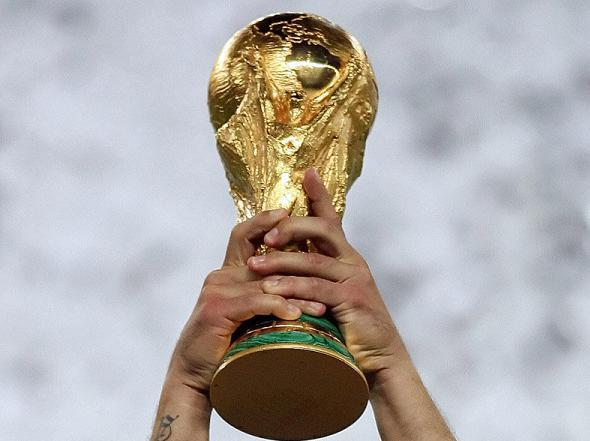
\includegraphics[width=0.6\textwidth]{Pictures/wm}
	\end{figure}
\end{frame}

\begin{frame}
	\frametitle{Table of contents}
	\tableofcontents
\end{frame}

\section{}
\begin{frame}
	\hfill
	\begin{beamercolorbox}[shadow=true, rounded=true, wd=10cm]{presinative}
		\centering
		\Large{\textbf{Thank you for your attention!}}
	\end{beamercolorbox}
	\hfill
\end{frame}

\end{document}
